The analysis of facial expressions constitutes a critical and complex portion of our non-verbal social interactions. Therefore, over the past years the computer science community has developed different methodologies or strategies to automatically analyze the facial expression \cite{Fasel1999}. Facial expression analysis is one of the most difficult and interesting problems in computer vision due to variability in shape and texture of the face. These variations are caused by some factors such as pose, illumination changes and occlusion. It is important to consider that facial expression recognition is different from facial expression analysis; the first is focused on classification of the structure of the face into a set of general emotions, see Figure \ref{fig:BasicEmotions}(A). The second focuses on meassuring how these emotions are produced in the face (mainly through facial muscles deformation analysis), see Figure \ref{fig:BasicEmotions}(B).

The analysis of human facial expressions has huge implications in areas like psychology, since, according to Ekman~\cite{Hager1979}, through this, it can not only be classified into one of the general seven emotions but also how they are generated. The corner stone for this is the symmetry of the facial muscles activity, which by its analysis it can be found whether an emotion is natural or not.

\begin{figure}[h]
    \centering
    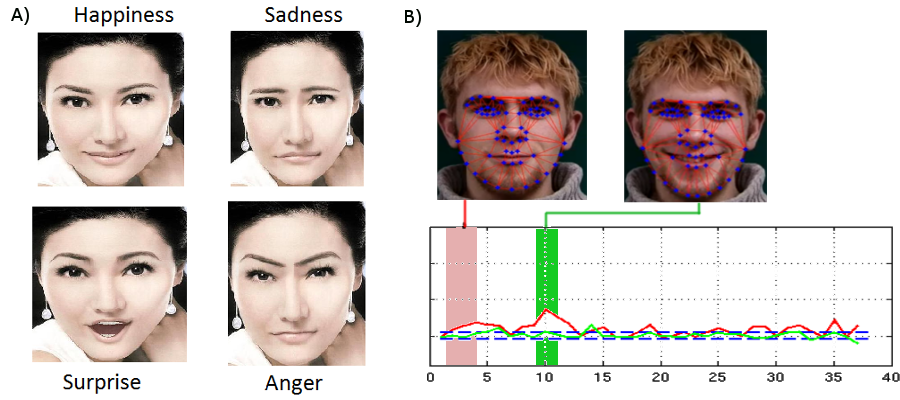
\includegraphics[scale=0.4]{images/emotionsAndGraphics1.png}
    \caption[Basic human emotions and Facial gesture analysis]{(A) Basic human emotions. (B) Facial gesture analysis. Emotion is a complex psychophysiological experience of an individual's state of mind as interacting with biochemical (internal) and environmental (external) influences}
    \label{fig:BasicEmotions}
\end{figure}

In computer vision and artificial intelligence (AI) there are many sub-problems related to facial emotion recognition such as: pose variations, people constantly moving their head in different angles; illumination changes, different environments with different illumination conditions; occlusion, which occurs when an object is in front of the face difficulting the analysis feature extraction task; background complexity, multiple objects in the environment with non-uniform background contrast; finally, image resolution which affects the accuracy of the tracking/recognition process. Besides, from the computational point of view, this problem implies the classification of facial motion or facial structure deformation into abstract representations completely based on visual information.

\subsection{Basic concepts}

Computational facial analysis methods can be classified in deformation extraction methods and motion extraction methods \cite{Fasel1999}:
\begin{description}
\item[Motion extraction:] these approaches focus on facial changes presented as consequence of facial expressions.
\item[Deformation extraction:] these approaches work with a neutral face images or face models for extract relevant facial features not caused by wrinkles or accidents.
\end{description}

The main difference between them is that deformation-based methods can be applied to image sequences, in the second case, the analysis can be applied to both single images and image sequences by processing frames independently. However, deformation-based feature extractors miss low-level directional motion information, i.e. they cannot reconstruct pixel motion. Although face motion can be inferred by using facial feature models it requires extra computation time to achieve it.

In both cases, facial features may be processed holistically (the faces are analyzed as a whole) or locally (focusing on features from specific areas).These approaches are focused on the extraction and analysis of two types of facial features \cite{Fasel1999}:
\begin{description}
\item[Intransient facial features:] always are in the face and could be deformed by facial expressions, for example, eyes, eyebrows and mouth.
\item[Transient facial features:] consider wrinkles and bulges in the face, for example, when the people open and close their eyes or mouth, face changes.
\end{description}

In both cases, the success of the technique depends on the capacity to segment the face from background. The correct segmentation allows an accurate extraction of points of interest from the faces. To do it, facial processing may take place either holistically, or locally, by focusing on facial features or areas that are prone to change with facial expressions. The task of separating the face from the background is done through segmentation, which allows the isolation of transient and intransient features within the face, that can be used to separate faces of interest from the background.

\subsection{Facial gestures analysis methods}
Facial gesture analysis is a challenging task and it has several application related to human interaction and computers. Traditionally, facial gestures recognition classifies the expressions into seven general emotions (anger, happiness, fear, sadness, contempt, disgust, surprise), in contrast, the facial expression analysis involves the reconstruction of facial motion, considering this way the facial muscle periods of motion between one gesture and another. In this cases it is necessary a robust classification and tracking technique of face gestures and head position \cite{Cinar01}.

There are three main steps for working in facial gestures recognition: face detection, extraction of facial gestures information and classification of the information extracted. As it was previously stated, the methods for facial gesture analysis can be grouped in deformation extraction and motion extraction.

\subsection{Review of Deformation and Motion Extraction Methods}
Over last years researchers have developed many approaches and models for face recognition and analysis with good results by using both deformation and motion extraction approaches. Although, the election of an specific technique relies on the characteristics of a certain problem. Deformation extraction have been successfully used to solve emotion recognition tasks, since they can be used to analyze single images. However, if the problem consists in analyzing a sequence of images to extract the \emph{motion} (caused by muscles actions) of different regions in the face while making a gesture, the motion extraction techniques are ideal to this goal, since they have been applied to evaluate the motion produced in areas like eyes or mouth, by using a model generated a priori.

In general, motion techniques uses either 2D or 3D information. Typically, 2D based techniques are more used due to their fastness, product of a reduced dimensionality of the information. Nevertheless,  a very large training data sets is needed to model the angular variations and illumination changes. In the case of 3D based approaches, the accuracy reached is higher than 2D based ones \cite{Fang2012}, since they are rotation invariant, although their sensitiveness to illumination changes remains.

In the case of facial expression analysis, precision is more important than processing speed, since the analysis can be carried on offline. Considering that, 3D based techniques are more relevant to solve the problem; especially those approaches with local oriented processing, since they allow analyzing information from specific points in the face (opposed points in the face are required in order to analyze the symmetry).

\subsection{3D based local analysis techniques}
As it was previously stated, the main difference about these techniques is the way they process information. Holistic approaches considers the whole image to extract motion vectors, which could be used for extracting general information about the motion of the face; still to increase the accuracy of facial expressions analysis requires the motion interpretation of specific regions in the face. On this line, there are several techniques in the state of the art (see Table \ref{tb:3DLocalTechniques}) that focuses on specific regions in the face:

\begin{table}[h]
\scriptsize
%\footnotesize
\begin{center}
\begin{tabular}{||p{2.7cm}|p{2.0cm}|p{2.0cm}|p{2.0cm}|p{1.5cm}|p{1.5cm}|p{1.5cm}||} \hline \hline
Reference & Sequences & Landmarks & Database & Expr. Types & R.P. (\%) \\ \hline \hline
\normalsize{Yin \cite{Yin2006}} & 2D + 4D & 64 semi-auto & BU-3DFE & 6 & 80.2 \\ \hline \hline
\normalsize{Wang \cite{Wang2007}} & 2D + 3D & 58 auto & Private & 4 & 83.0 \\ \hline \hline
\normalsize{Sun \cite{SunFer2008}} & 2D + 4D & 83 auto & BU-4DFE & 6 & 80.9 \\ \hline \hline
\normalsize{Rosato \cite{Rosato2008}} & 2D + 4D & 22 auto & BU-3DFE, BU-4DFE & 7 & 80.1 \\ \hline \hline
\normalsize{Zhao \cite{Zhao01}} & 2D + 3D & 19 manual & Bosphorus & 7 & 94.2 \\ \hline \hline
\normalsize{Tsalakanidou \cite{Tsalakanidou2010}} & 2D + 4D & 81 auto & Private & 5 & 85.0 \\ \hline \hline
\end{tabular}
\end{center}
\caption[Methods for $3D/4D$ Facial Expression Analysis]{Methods for $3D/4D$ Facial Expression Analysis (\footnotesize{Headers: \textbf{Sequences} denotes the dimensions of the images where 2D denotes whether the method makes use of the 2D texture associated with the 3D data and 4D denotes whether the method uses temporal information from a sequence of 3D data; \textbf{Database} denotes the database from which a subset was selected; \textbf{R.P.} denotes reported performance, which is the average recognition rates}).}
\label{tb:3DLocalTechniques}
\end{table}

The approaches described previously have the ability to perform facial expressions analysis considering 3D information. These techniques can be classified into two main groups, depending on the labelling mechanism: automatic and manual. In the case of the automatic labelling mechanisms, authors have used automatic fitting techniques to extract different numbers of facial regions of interest (22- \cite{Rosato2008} and 58 \cite{Wang2007}). In the case of the manual labelling mechanisms, the existing techniques require off line characterization of the facial regions of interest. As it can be seen in Table \ref{tb:3DLocalTechniques}, there is a difference on the percentage of recognition achieved by techniques in these two categories: methodologies designed to manual labelling reached as top a 94.2\% compared to 85.0\%. Also from the table \ref{tb:3DLocalTechniques}, there is no clear difference about the number of points to be used (but the higher the number of points is the higher computational complexity as well as a higher recognition rate). Although it remains to review, automatic labelling techniques are more desirable for facial expression analysis problems, since they reduce the dependance from user interaction.
